\documentclass[12pt, a4paper]{article}

% Required Packages
\usepackage[utf8]{inputenc}
\usepackage{graphicx}
\usepackage{geometry}
\usepackage{fancyhdr}
\usepackage{hyperref}
\usepackage{subcaption}
\usepackage{float}
\usepackage{amsmath}

% Page Geometry
\geometry{top=1in, bottom=1in, left=1in, right=1in}

% Set the graphics path to the subfolder where you will place the images and PDF
\graphicspath{{Images/}}

% Header and Footer Setup
\pagestyle{fancy}
\fancyhf{}
\rhead{Grid-Forming Inverter: Droop Control}
\lhead{Abd El-Rhman Muhammad Saad 19017058}
\cfoot{\thepage}

% Hyperlink Setup
\hypersetup{
	colorlinks=true,
	linkcolor=blue,
	filecolor=magenta,      
	urlcolor=blue,
}

\begin{document}
	
	% ---------------- TITLE PAGE ---------------- %
	\begin{titlepage}
		\begin{flushleft}
			\begin{minipage}{0.15\textwidth}
				
\includegraphics[width=\textwidth]{logo.png} 
			\end{minipage}%
			\hspace{0.3cm}
			\begin{minipage}{0.7\textwidth}
				{\scshape\large Alexandria University} \\[0.1cm]
				{\scshape\normalsize Faculty of Engineering} \\[0.1cm]
				{\scshape\normalsize Electrical Engineering Department}
			\end{minipage}
		\end{flushleft}
		
		\vspace{2.0cm}
		\centering
		{\Huge\bfseries Microgrid Control Systems \par}
		\vspace{0.4cm}
		{\Large\bfseries Grid-Forming Inverter System: Droop Control and Power Management \par}
		
		\vspace{1.0cm}
		{\Large\itshape Prepared by:\par}
		\vspace{0.2cm}
		{\Large \textbf{Abd El-Rhman Muhammad Saad Muhammad}\par}
		{\large \textbf{ID:} 19017058\par}
		
		\vfill
		{\large \textbf{Simulink Model Link:}\par}
		{\normalsize \href{https://github.com/Abd-El-Rhman-Saad/grid-forming-inverter-simulation}{Click here to access the Simulink Model on GitHub}}\par
		
		\vfill
		{\large \textbf{Date:} May 2026 \par}
	\end{titlepage}
	
	\newpage
	
	\begin{abstract}
		This report presents the comprehensive design, mathematical modeling, and MATLAB/Simulink simulation of a Grid-Forming Voltage Source Inverter (GFM-VSI). Unlike traditional grid-following inverters that inject current into a stiff grid, grid-forming inverters act as controlled AC voltage sources that establish the local grid voltage and frequency. The implemented system employs a Droop Control strategy ($P-\omega$ and $Q-V$) to autonomously share active and reactive power without relying on external communication. Furthermore, a cascaded multi-loop control architecture operating in the synchronous reference frame ($dq0$) is implemented to track the generated voltage reference. In the simulation, the inverter forms a stable AC voltage and its mean active power settles at 20 kW, equal to the reference $P^*$, within about one second.
	\end{abstract}
	
	\newpage
	\tableofcontents
	\newpage
	
	% ---------------- SECTION 1: SYSTEM OVERVIEW ---------------- %
	\section{System Specifications and Architecture}
	The simulated system comprises a Two-Level Voltage Source Inverter powered by a stiff 800V DC source. The inverter interfaces with the 400V (line-to-line RMS), 50Hz AC grid through a third-order LCL filter, which provides high harmonic attenuation for the 5 kHz switching frequency components.
	
	The system architecture is divided into three main sub-systems: (1) Power and Droop Control for reference generation, (2) Inner Control Loops for voltage/current tracking, and (3) Signal Transformation for coordinate mapping. Table 1 summarizes the core system parameters. In the model, the inverter is connected through the LCL filter to a three-phase source (400 V, 50 Hz) with a source impedance of $0.893\,\Omega + 16.58\,\text{mH}$.
	
	\begin{table}[H]
		\centering
		\caption{Grid-Forming Inverter System Parameters}
		\begin{tabular}{lc}
			\hline
			\textbf{Parameter} & \textbf{Value} \\
			\hline
			Nominal AC Grid Voltage ($V_{LL}$) & 400 V (rms) \\
			Peak Phase Voltage Reference ($V^*$) & 326.7 V \\
			Nominal System Frequency ($f^*$) & 50 Hz \\
			Nominal Angular Frequency ($\omega^*$) & $100\pi$ rad/s \\
			DC Link Voltage ($V_{DC}$) & 800 V \\
			Active Power Reference ($P^*$) & 20 kW \\
			Frequency Droop Coefficient ($m_p$) & $5 \times 10^{-5}$ \\
			Voltage Droop Coefficient ($n_q$) & $5 \times 10^{-6}$ \\
			LCL Inverter-Side Inductor & 3 mH \\
			LCL Filter Capacitor & 220 $\mu$F \\
			LCL Grid-Side Branch & 0.2 $\Omega$ + 1 mH \\
			Switching Frequency & 5 kHz \\
			\hline
		\end{tabular}
	\end{table}
	
	\begin{figure}[H]
		\centering
		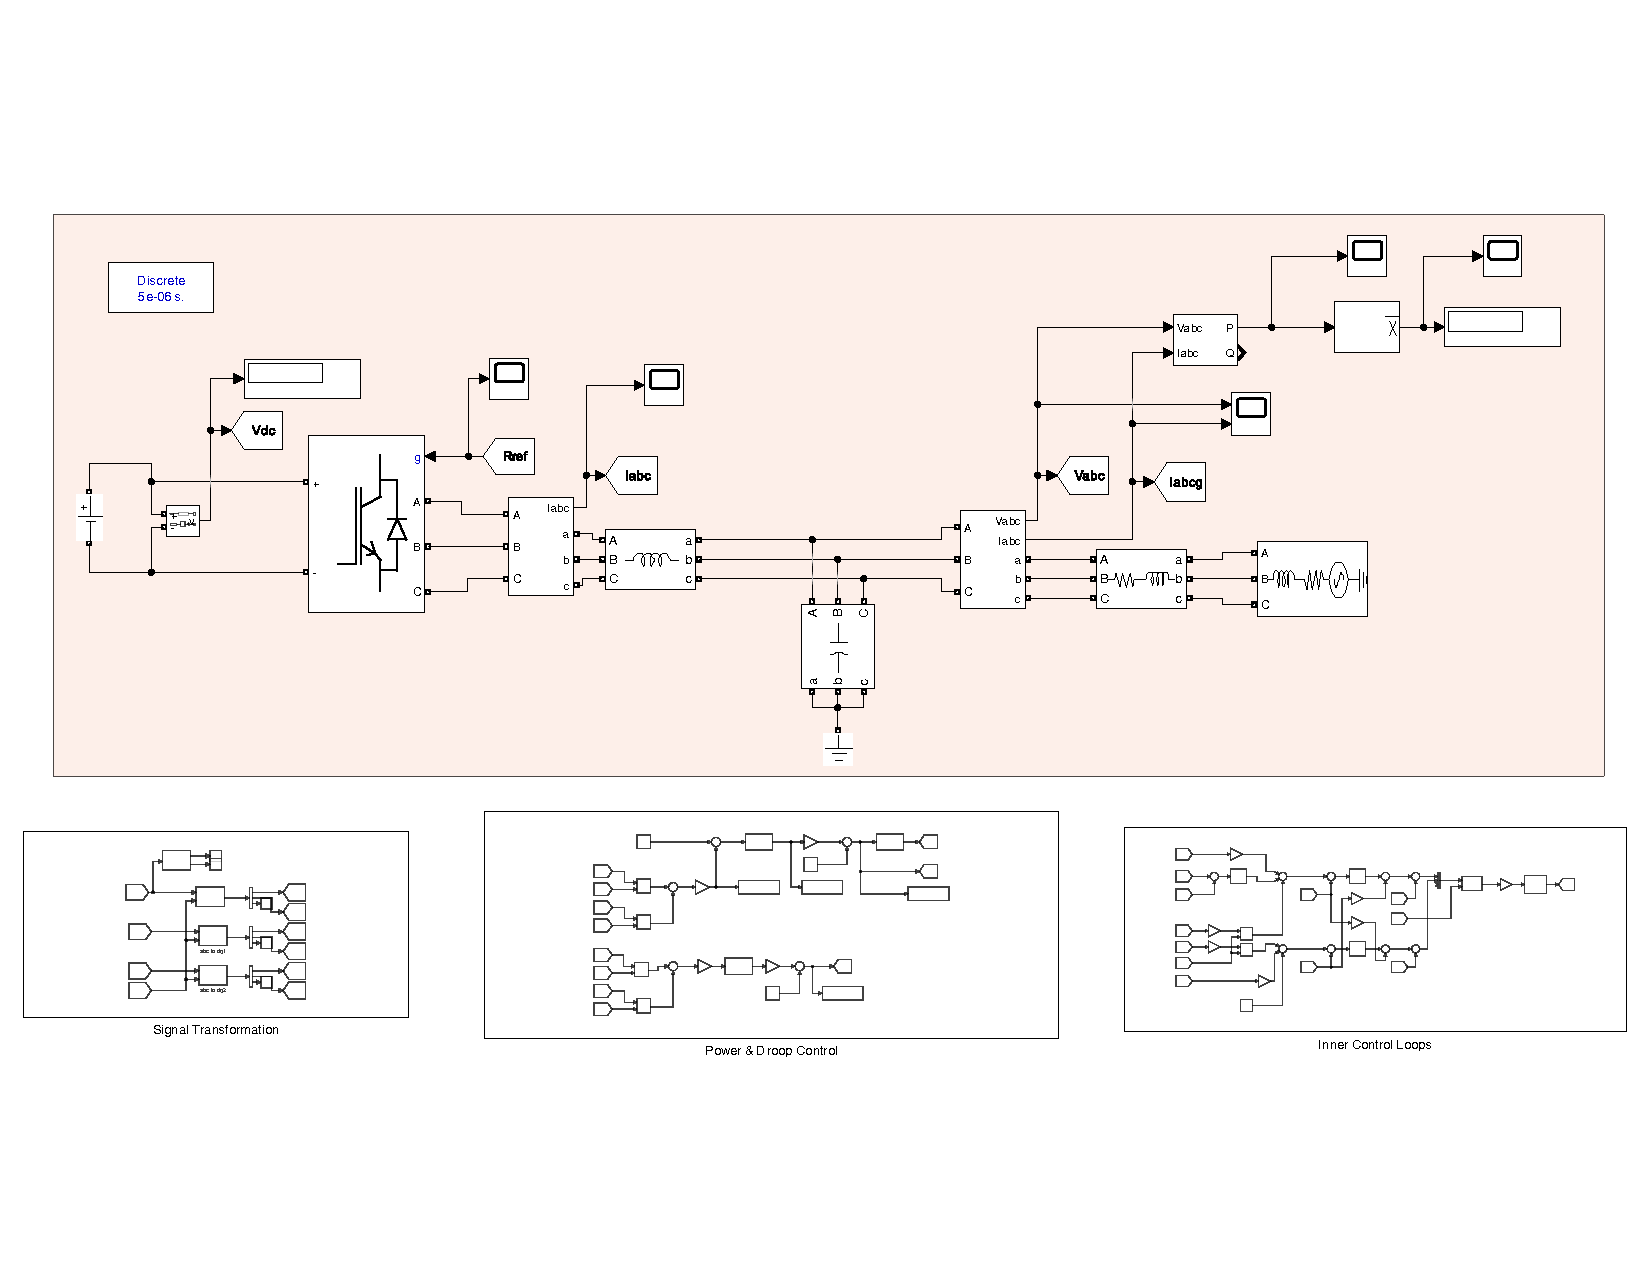
\includegraphics[page=1, width=\textwidth]{Full_Sys.pdf}
		\caption{Overall Architecture of the Grid-Forming Inverter System.}
	\end{figure}
	
	\newpage
	% ---------------- SECTION 2: CONTROL STRATEGY ---------------- %
	\section{Advanced Control Strategy}
	The control structure of the Grid-Forming Inverter mimics the physical dynamics of a traditional Synchronous Generator (SG). It generates its own internal voltage angle and magnitude using outer power droop loops, followed by fast inner voltage and current loops.
	
	\subsection{Power Calculation and Droop Control}
	The outer control loop (shown in Figure 2) is responsible for calculating the instantaneous active ($P$) and reactive ($Q$) powers using the measured $d$ and $q$-axis voltages and currents:
	
	\begin{equation}
		P = \frac{3}{2} (v_d i_{d} + v_q i_{q}), \quad Q = \frac{3}{2} (v_q i_{d} - v_d i_{q})
	\end{equation}
	
	To eliminate high-frequency ripples and power oscillations, the calculated powers are passed through a first-order low-pass filter with a transfer function of $30 / (s + 30)$. 
	
	The filtered active power is then fed into the \textbf{Frequency Droop Controller} ($P-\omega$). This controller allows multiple parallel inverters to share active power by mimicking the mechanical speed governor of an SG:
	\begin{equation}
		\omega = \omega^* - m_p (P - P^*)
	\end{equation}
	Where $\omega^*$ is the nominal angular frequency ($100\pi$ rad/s) and $P^*$ is the nominal setpoint (20 kW). The continuous integration of the generated frequency ($\omega$) produces the internal phase angle ($\theta = \int \omega dt$) used for all $dq0$ transformations, completely eliminating the need for a Phase-Locked Loop (PLL) in steady-state grid-forming mode.
	
	Simultaneously, the filtered reactive power is fed into the \textbf{Voltage Droop Controller} ($Q-V$) to generate the internal voltage magnitude reference:
	\begin{equation}
		V_{ref} = V^* - n_q (Q)
	\end{equation}
	Where $V^*$ is the nominal peak phase voltage ($326.7\text{ V}$).
	
	\begin{figure}[H]
		\centering
		\includegraphics[page=3, width=0.9\textwidth]{Full_Sys.pdf}
		\caption{Power Calculation and $P-\omega$, $Q-V$ Droop Controllers.}
	\end{figure}
	
	\newpage
	\subsection{Cascaded Voltage and Current Loops}
	To ensure that the inverter accurately synthesizes the $V_{ref}$ calculated by the droop controller, a cascaded multi-loop architecture is implemented in the $dq0$ synchronous reference frame (Figure 3).
	
	
	\subsubsection{Inner Current Loop and Decoupling}
	The inner loop ($P = 100, I = 20000$) regulates the inverter output currents. Due to the rotating reference frame, a physical cross-coupling exists between the $d$ and $q$ axes. To guarantee independent control and prevent instability, \textbf{Feedforward Decoupling Terms} ($\pm \omega L \cdot i$) are added to the PI controller outputs. 
	
	The decoupled command voltages are converted back to the $abc$ frame to generate the final modulating signals ($U_{ref}$) sent to the PWM generator.
	
	\begin{figure}[H]
		\centering
		\includegraphics[page=2, width=0.75\textwidth]{Full_Sys.pdf}
		\caption{Cascaded Inner Control Loops showing PI controllers and Decoupling terms.}
	\end{figure}
	
	\subsubsection{Outer Voltage Loop}
	The voltage loop regulates the voltage across the filter capacitor. A Proportional-Integral (PI) controller tracks the error between the generated reference $V_{ref}$ (applied to the $d$-axis) and the actual capacitor voltage $V_d$. The $q$-axis voltage reference is strictly set to zero to align the voltage vector with the $d$-axis. The output of the voltage controllers serves as the reference currents ($I_d^*, I_q^*$) for the inner loop.
	
	\begin{figure}[H]
		\centering
		\includegraphics[page=4, width=0.45\textwidth]{Full_Sys.pdf}
		\caption{Signal Transformation Subsystem ($abc$ to $dq0$).}
	\end{figure}
	
	\newpage
	% ---------------- SECTION 3: SIMULATION RESULTS ---------------- %
	\section{Simulation Results and Analysis}
	The performance of the Grid-Forming Inverter was evaluated under steady-state and dynamic load sharing conditions.
	
	\subsection{Power Tracking and Droop Response}
	Figure 5 shows the response of the mean active power output. After initialization the power rises to a peak of about 21.5 kW (an overshoot of about 7.5\%) at $t \approx 0.5$ s, then settles at 20 kW, equal to the reference $P^*$, by about $t \approx 1$ s with no visible steady-state error. In steady state the inverter frequency equals the grid frequency, so the droop law of Eq. (2) returns $P = P^*$; during the transient the droop adjusts the internal frequency. 
	
	\begin{figure}[H]
		\centering
		\begin{subfigure}{0.8\textwidth}
			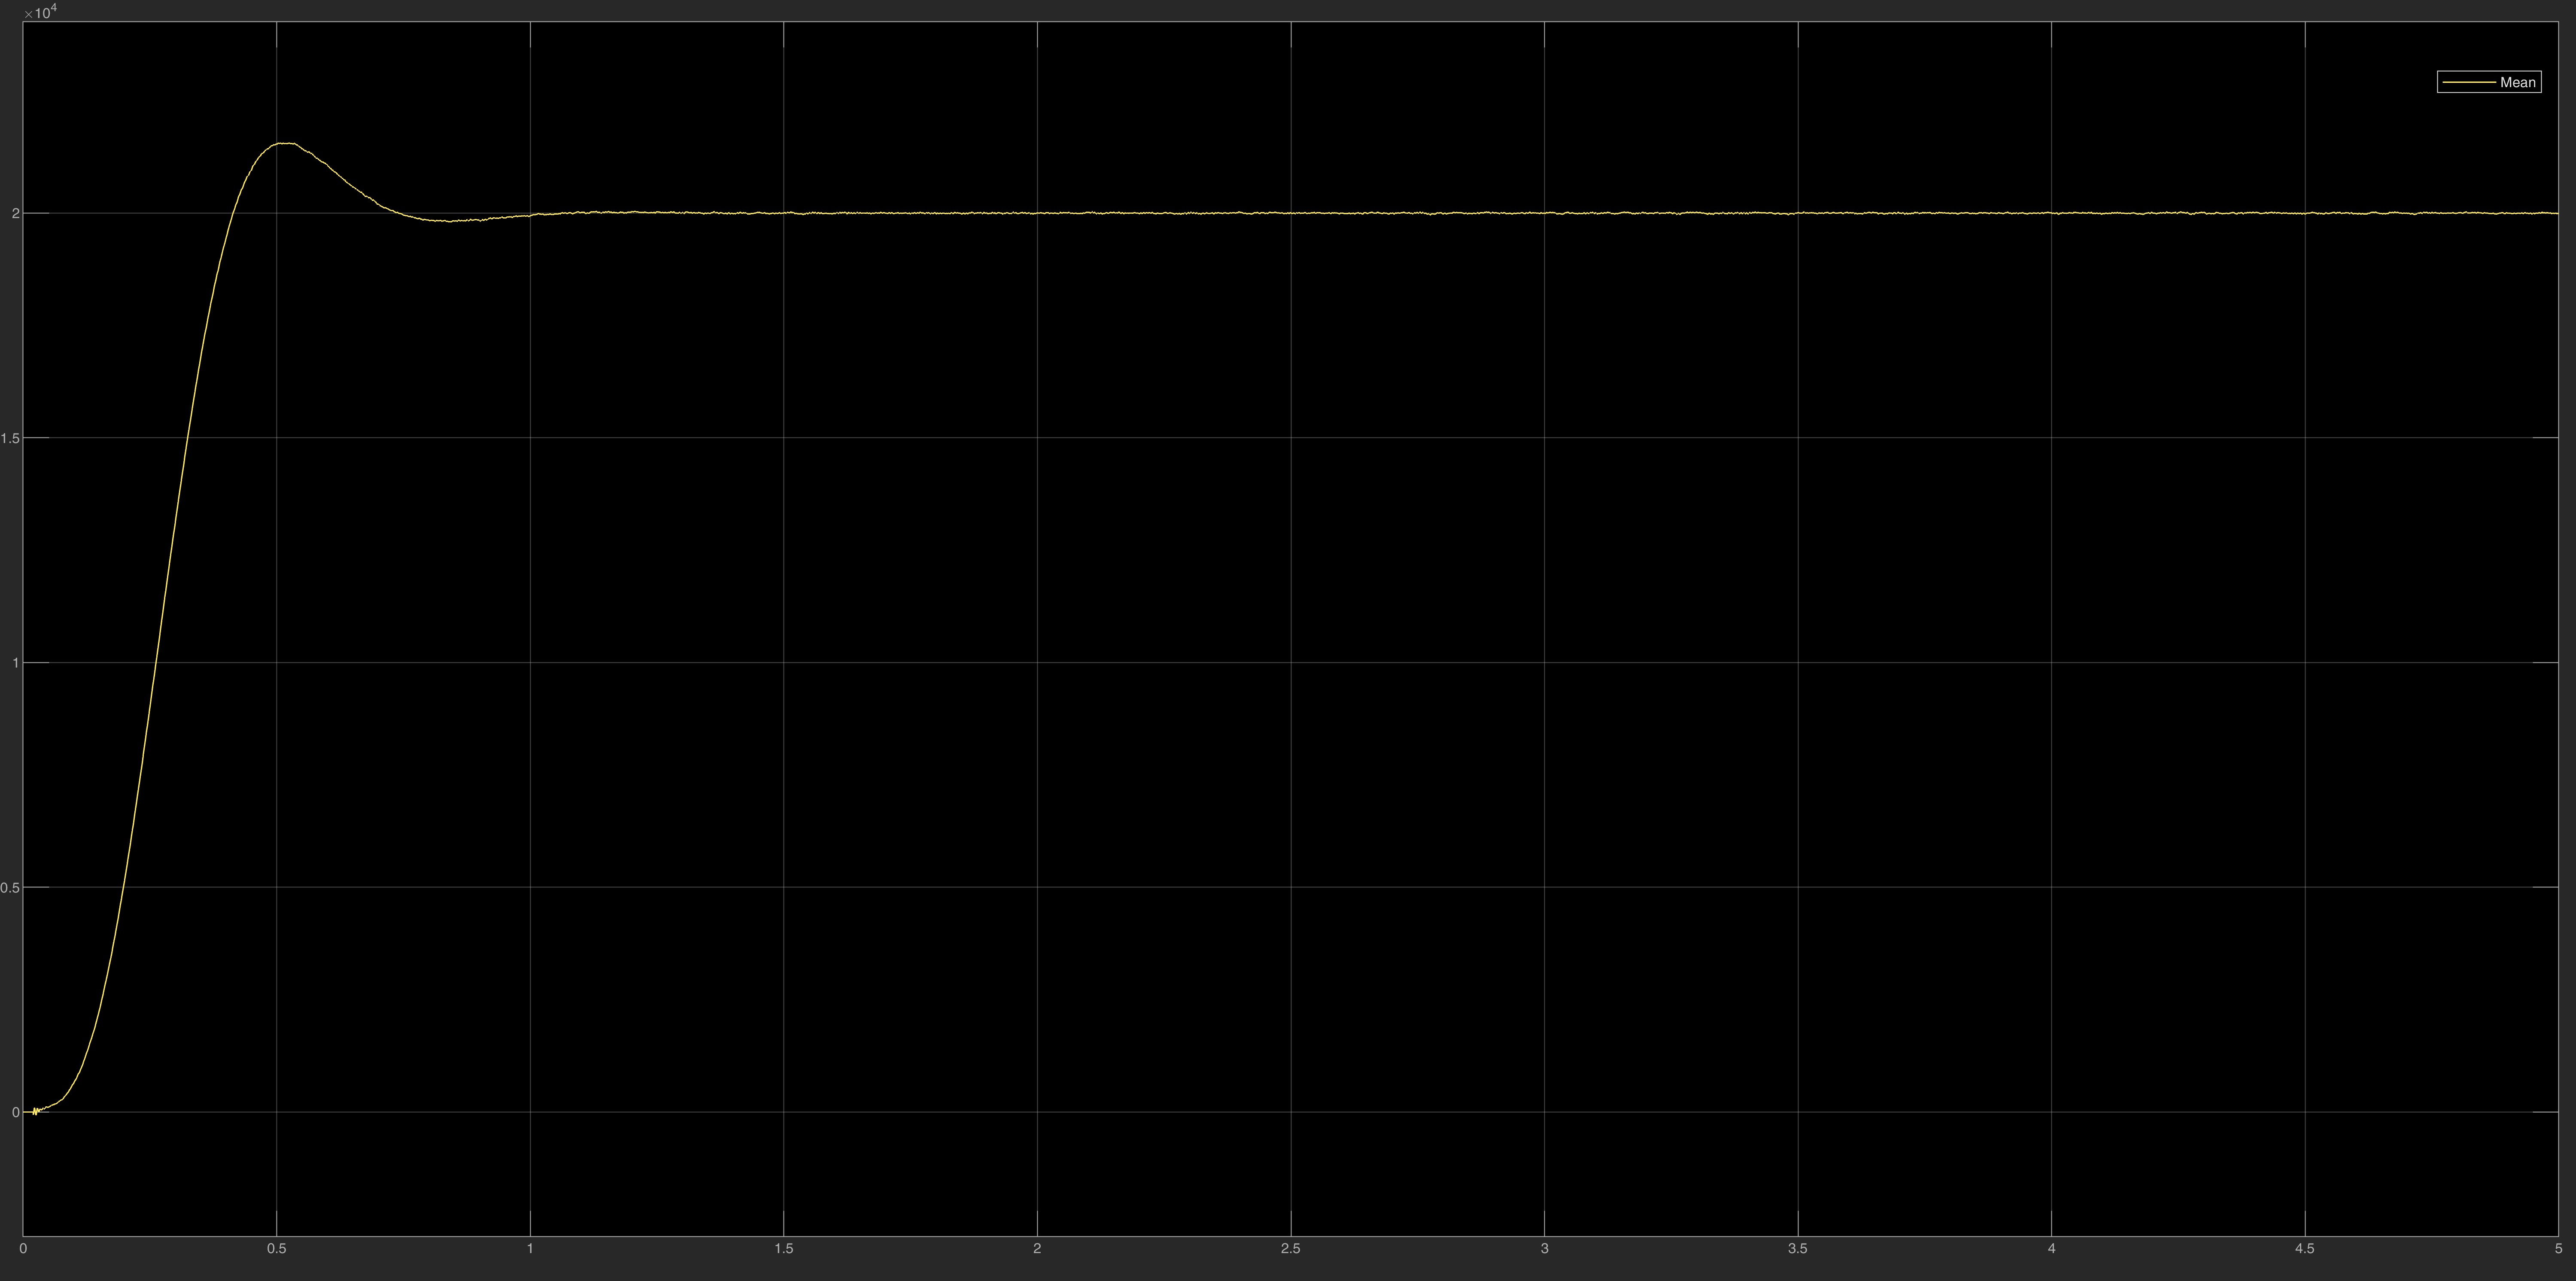
\includegraphics[width=\textwidth]{Scope1.jpg}
			\caption{Active Power Output Tracking}
		\end{subfigure}
		\vskip\baselineskip
		\begin{subfigure}{0.8\textwidth}
			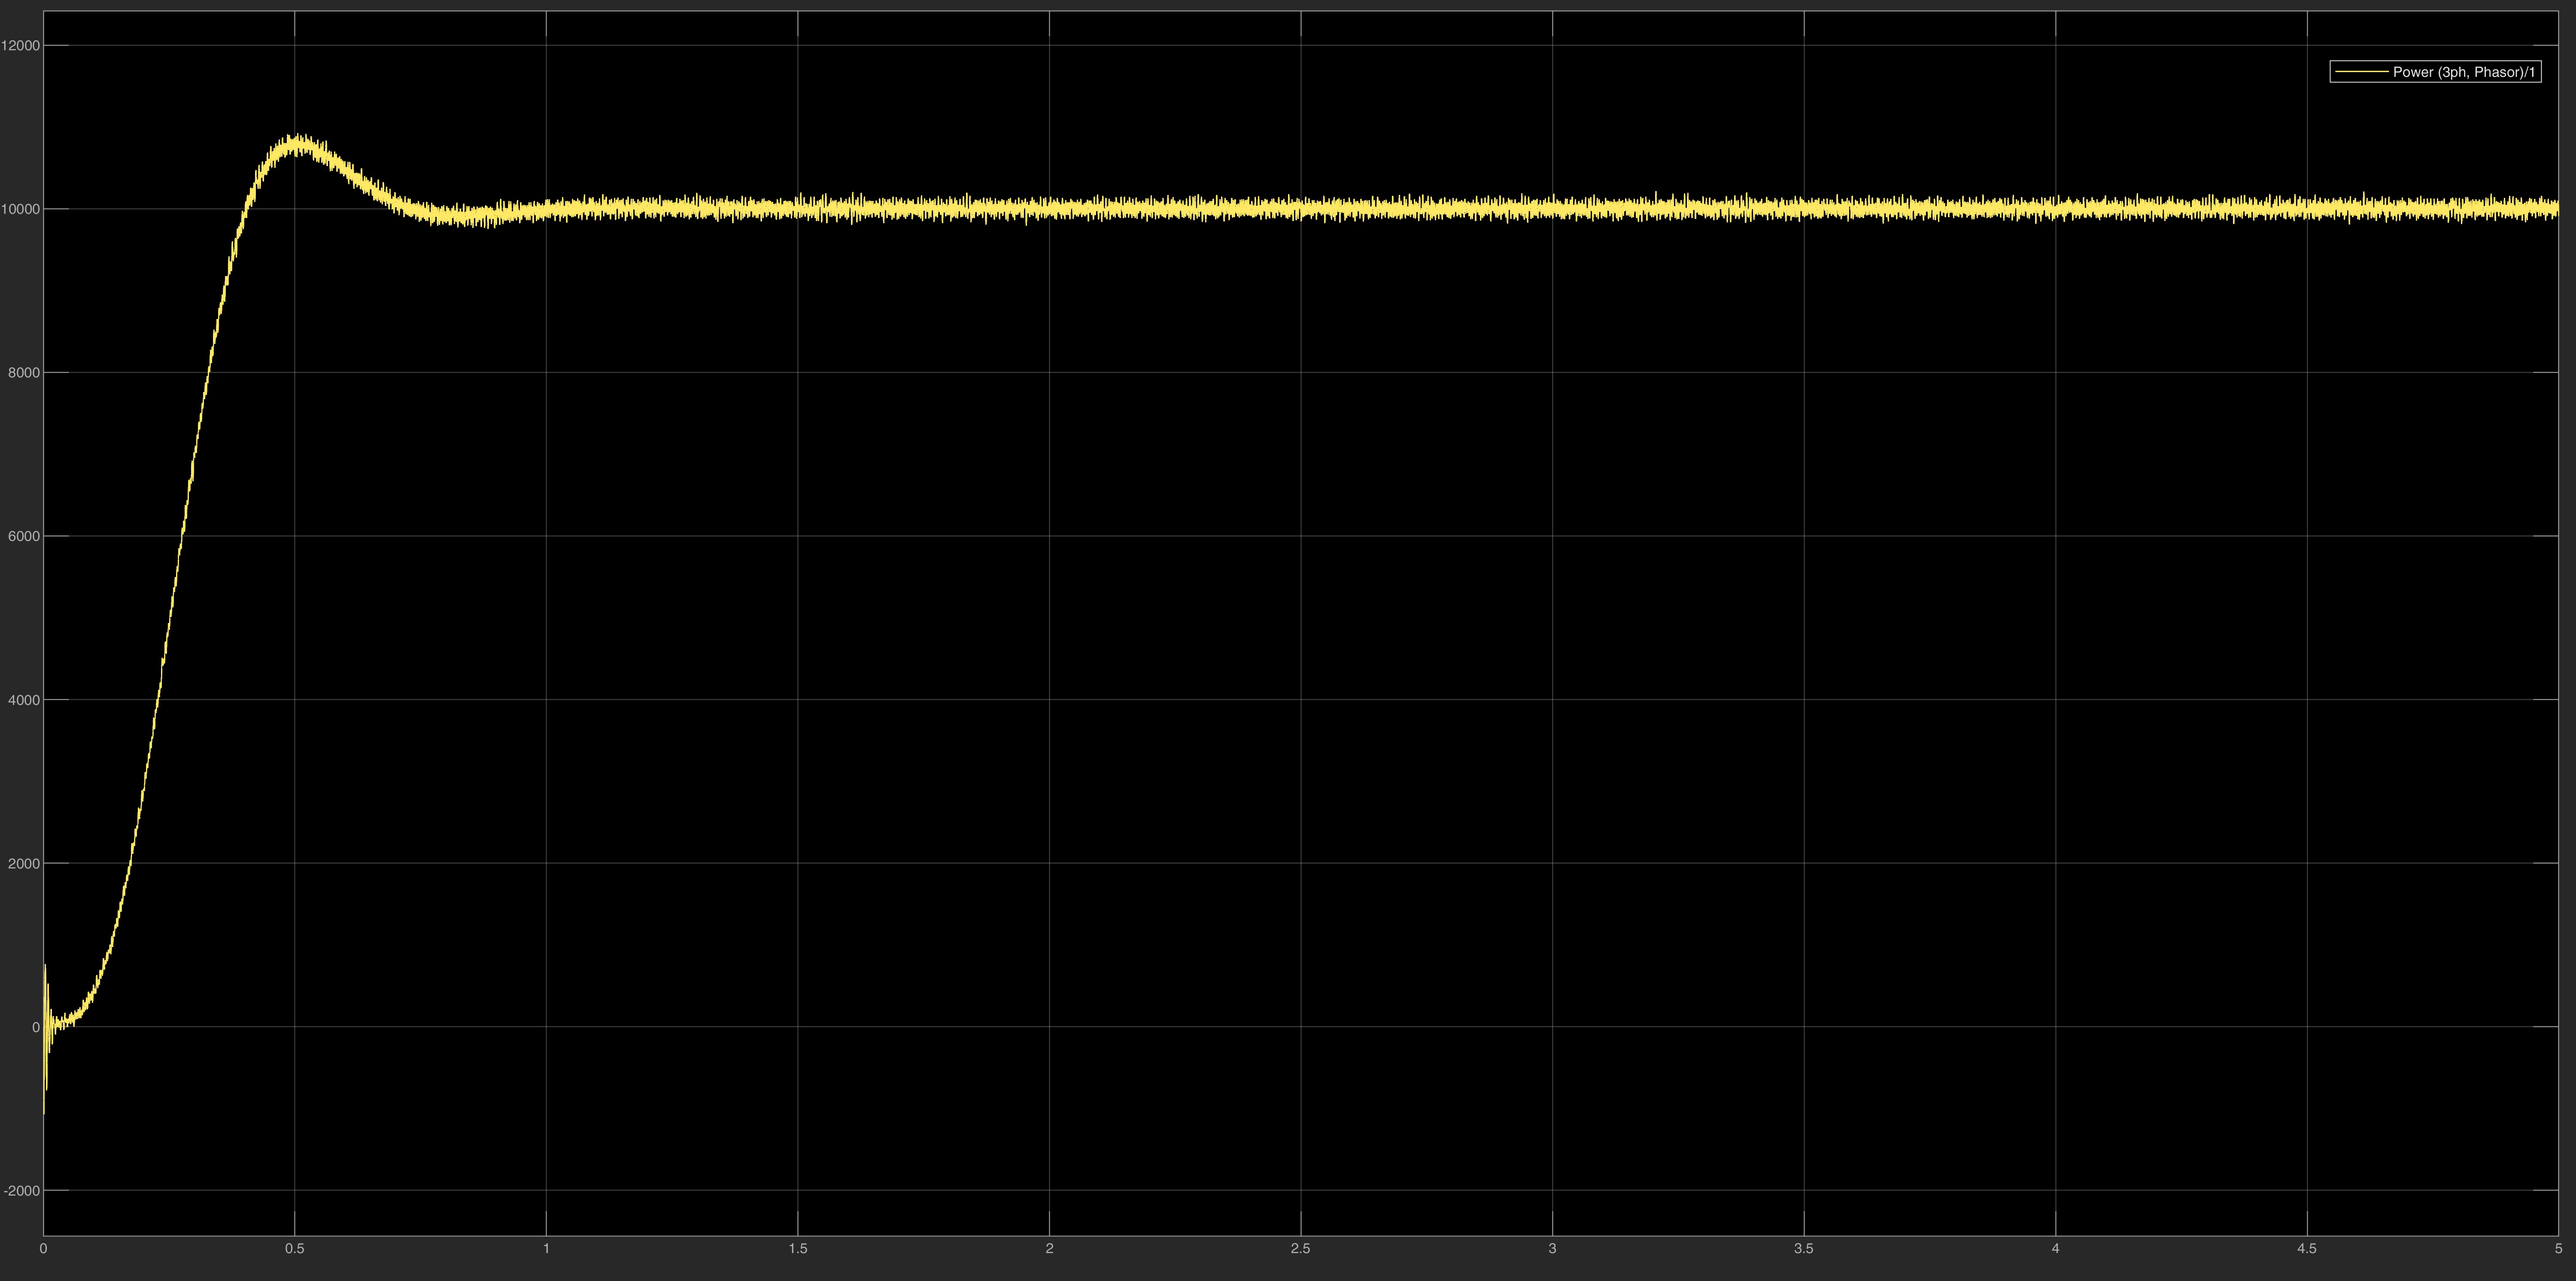
\includegraphics[width=\textwidth]{Scope2.jpg}
			\caption{Three-Phase Output Power Dynamics}
		\end{subfigure}
		\caption{Power response exhibiting stable tracking driven by the Droop Control loop.}
	\end{figure}
	
	\newpage
	\subsection{Voltage Quality and Inverter Waveforms}
	The inverter produces a sinusoidal output voltage at the AC interface. Figure 6 demonstrates the three-phase output voltage and current waveforms. The LCL filter together with the fast inner current PI loop attenuates the switching harmonics generated by the PWM mechanism (Figure 7).
	
	\begin{figure}[H]
		\centering
		\begin{subfigure}{0.85\textwidth}
			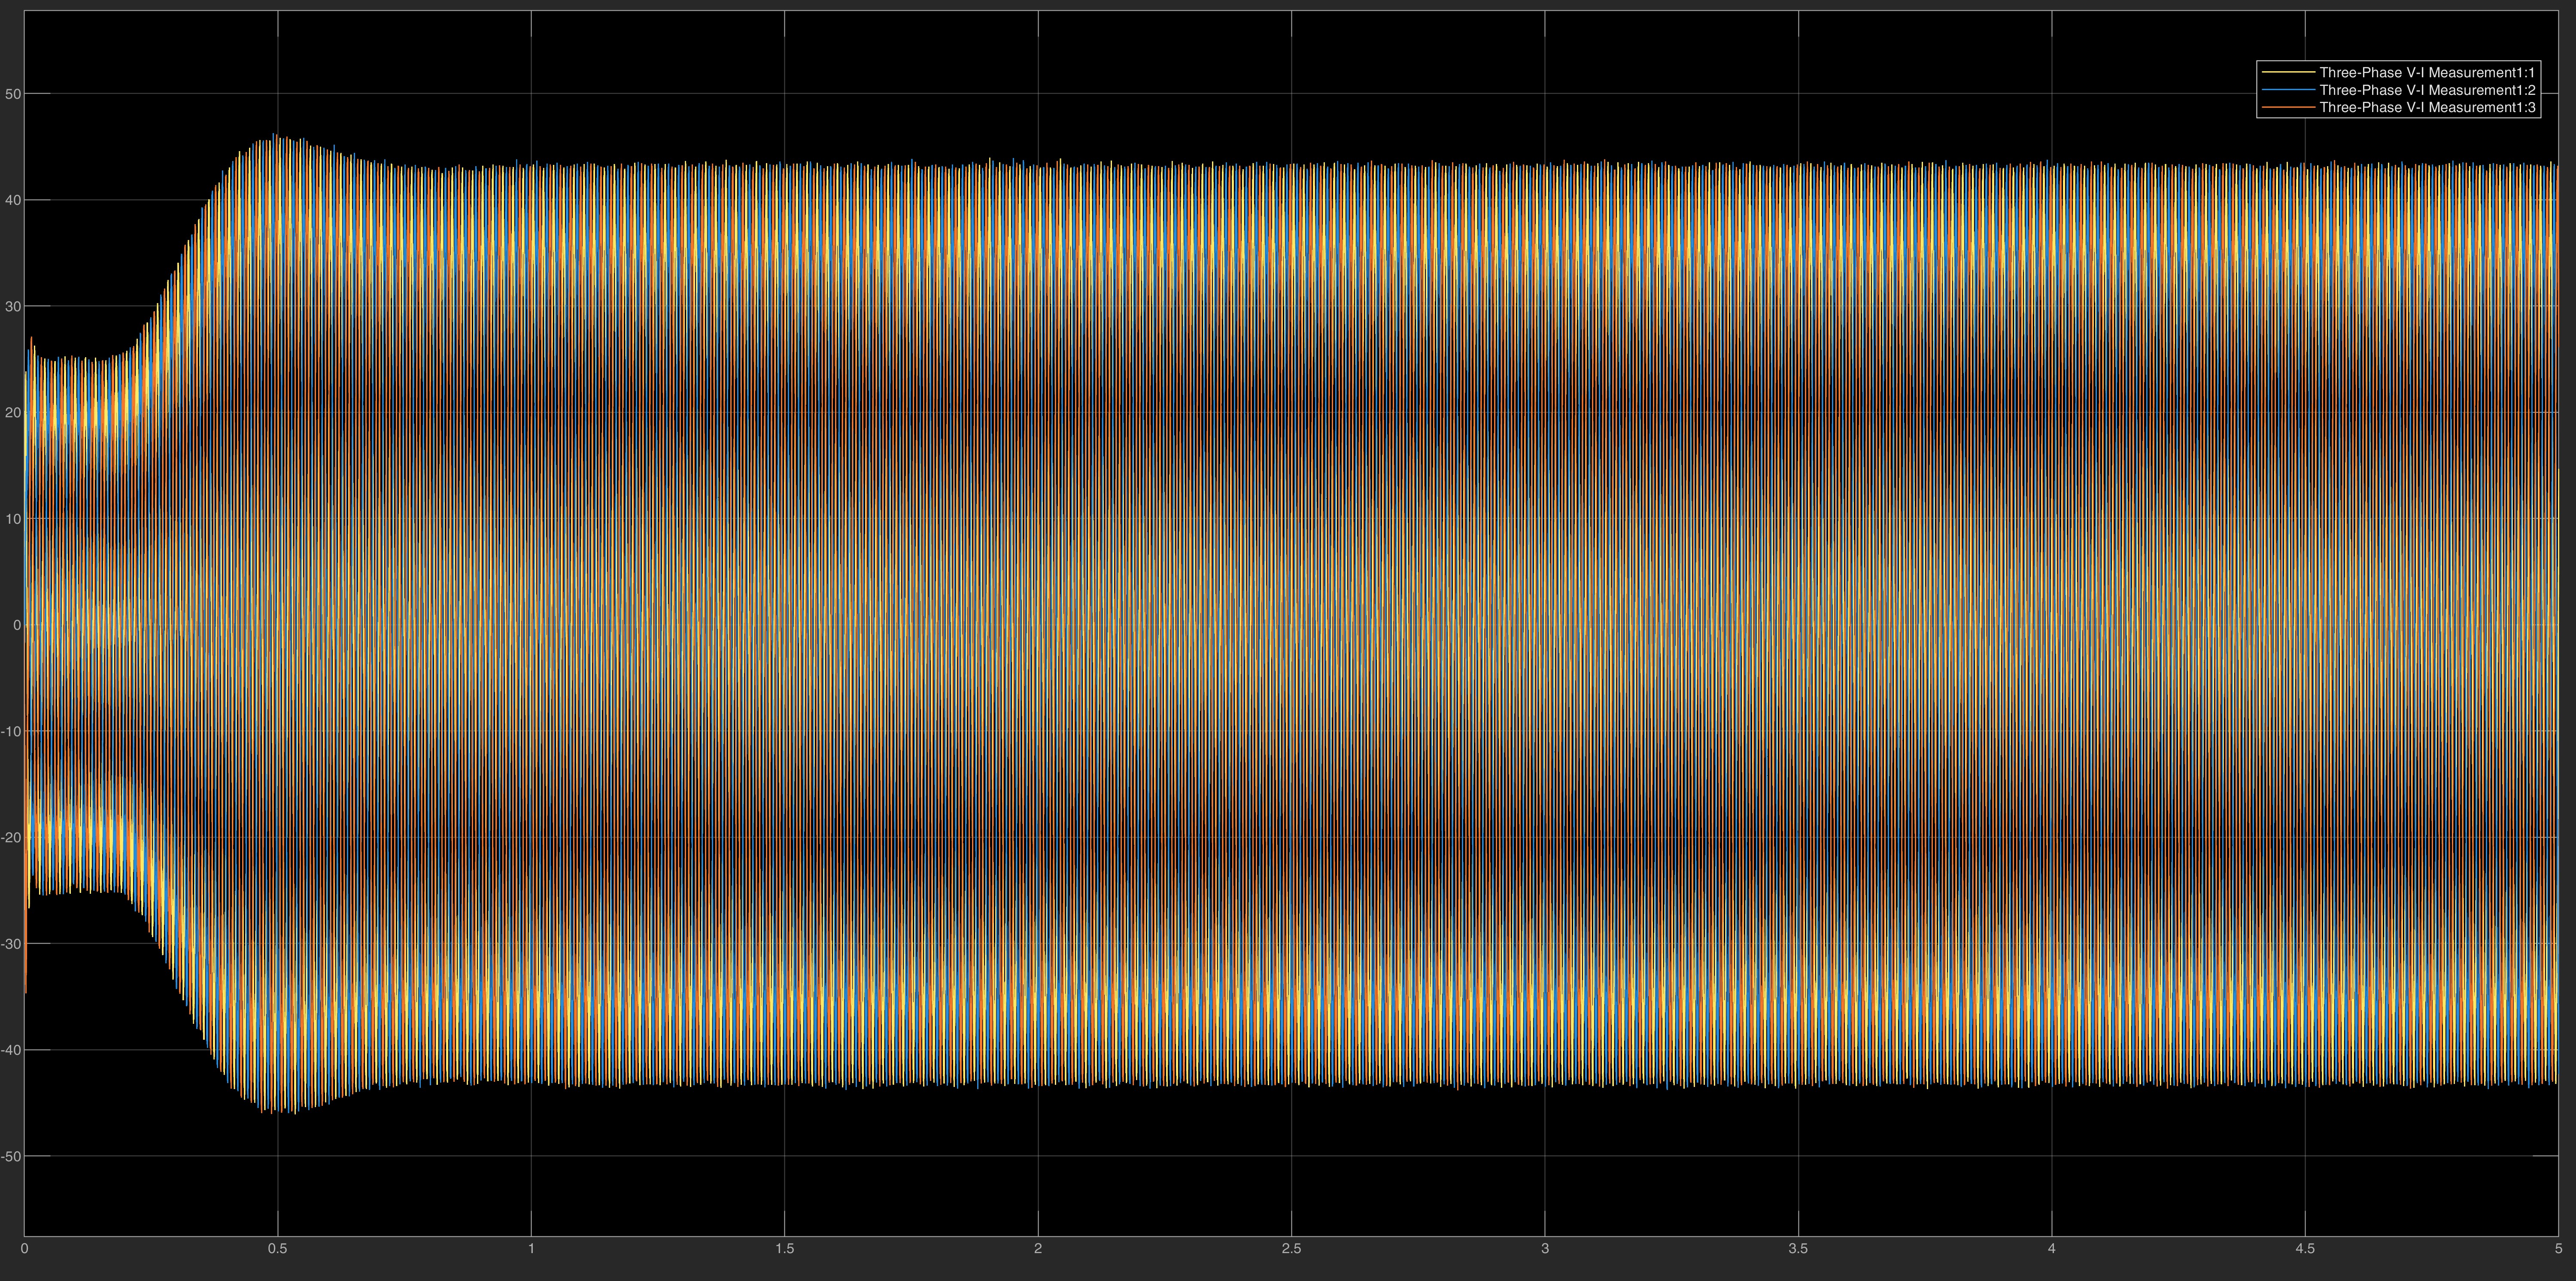
\includegraphics[width=\textwidth]{Scope4.jpg}
			\caption{Steady-state Three-Phase Waveforms}
		\end{subfigure}
		\vfill
		\begin{subfigure}{0.85\textwidth}
			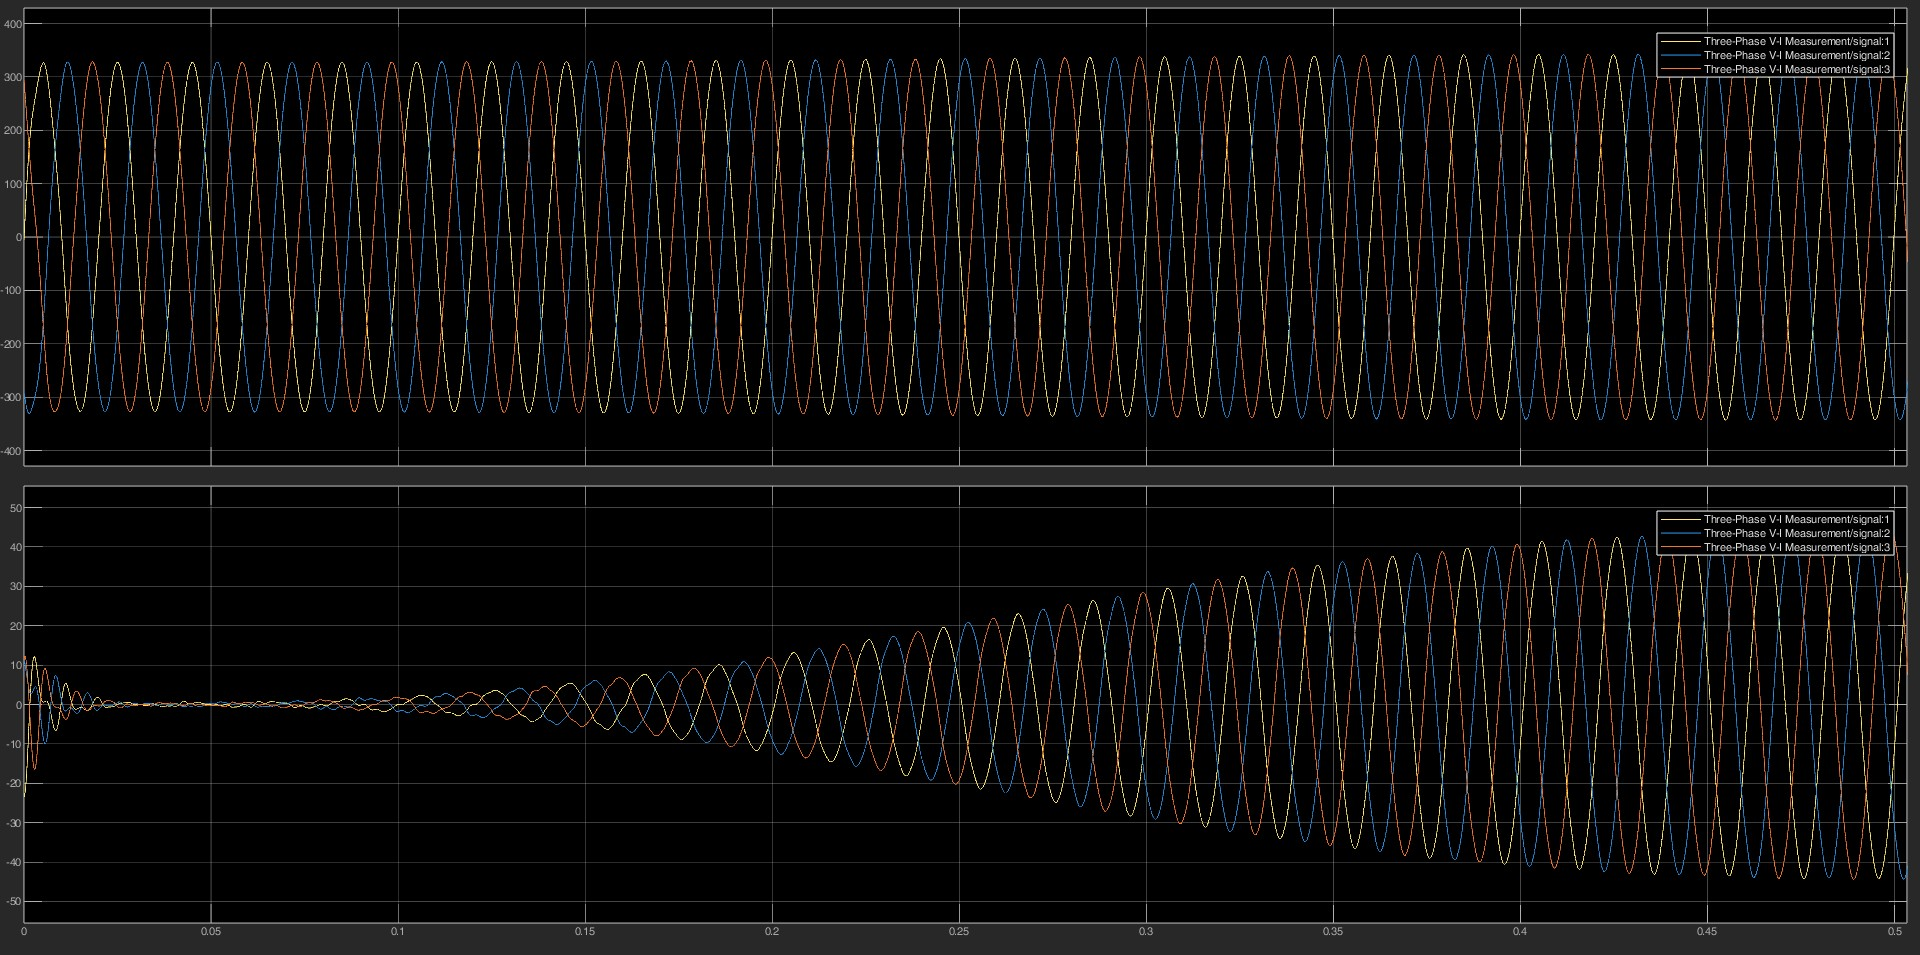
\includegraphics[width=\textwidth]{Scope_Zoomed.jpg}
			\caption{Zoomed-in view showing smooth sinusoidal waveforms}
		\end{subfigure}
		\caption{Generated Voltage and Current waveforms at the AC grid interface.}
	\end{figure}
	
	\begin{figure}[H]
		\centering
		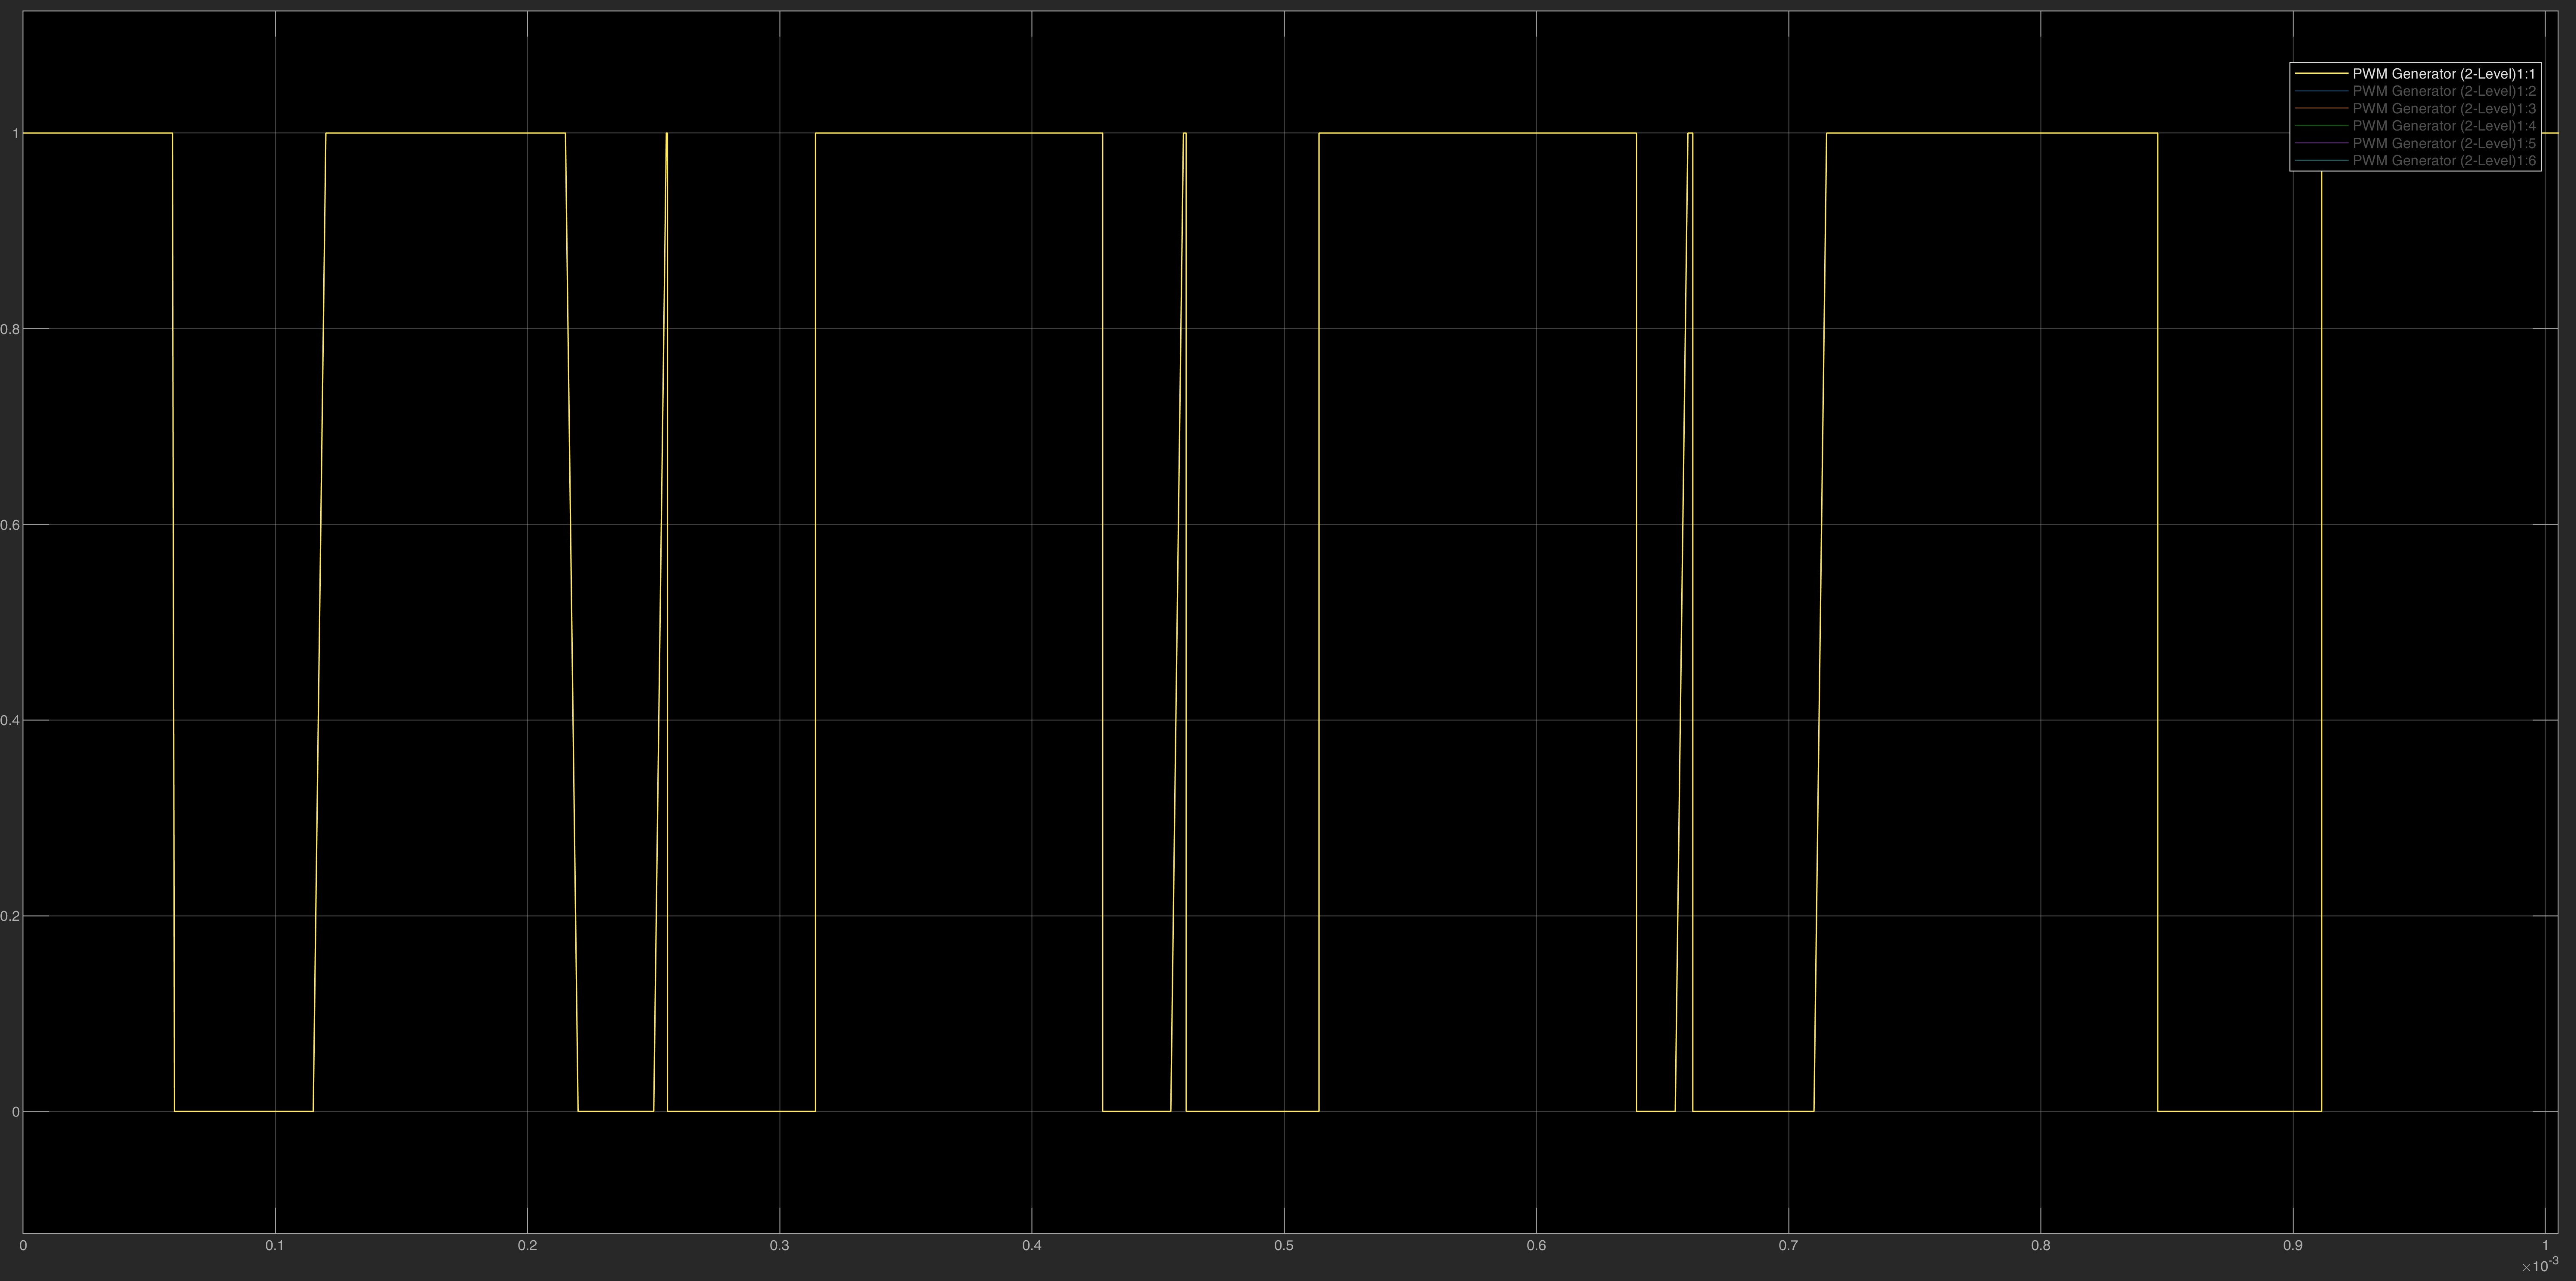
\includegraphics[width=0.7\textwidth]{Scope3_Zoomed.jpg}
		\caption{Zoomed-in view of the $5\text{ kHz}$ Pulse Width Modulation (PWM) signals.}
	\end{figure}
	
	\section{Conclusion}
	The design and simulation of the Grid-Forming Voltage Source Inverter were carried out in MATLAB/Simulink. The control architecture regulates the output voltage magnitude and frequency autonomously through droop control. The outer $P-\omega$ and $Q-V$ droop loops generate the internal angle and voltage reference, and the active power settles in a well-damped response. Furthermore, the $dq0$-based cascaded inner loops, fortified with decoupling terms, provide reference tracking with a sinusoidal output. Load-step response and power sharing between several inverters were not simulated and are the natural next steps toward isolated-microgrid operation.
	
\end{document}